\documentclass[tikz,border=10pt]{standalone}
\begin{document}
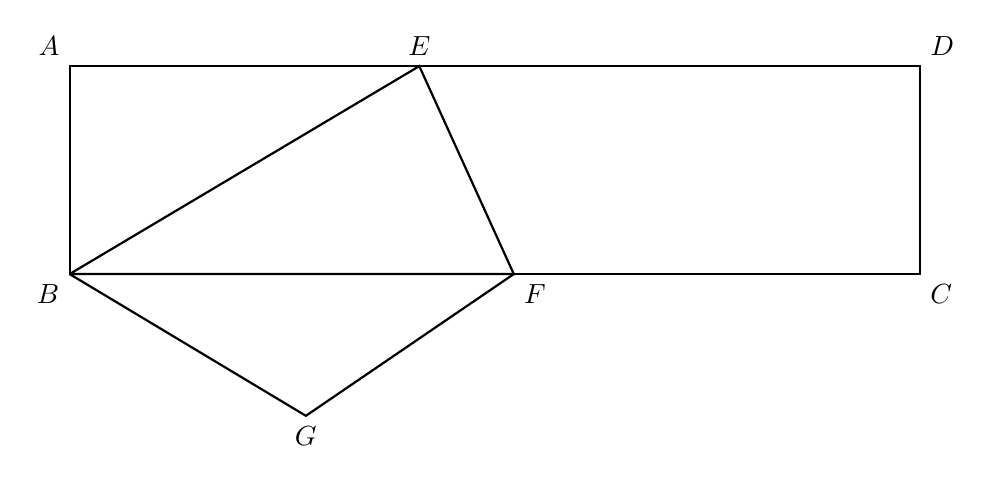
\begin{tikzpicture}[scale=1.2,thick]
\coordinate (A) at (0,3);
\coordinate (B) at (0,0.8);
\coordinate (C) at (9,0.8);
\coordinate (D) at (9,3);
\coordinate (E) at (3.7,3);
\coordinate (F) at (4.7,0.8);
\coordinate (G) at (2.5,-0.7);

\draw (A) -- (D) -- (C) -- (B) -- cycle;
\draw (B) -- (E) -- (F) -- (B);
\draw (B) -- (G) -- (F);

\node[above left] at (A) {$A$};
\node[below left] at (B) {$B$};
\node[below right] at (C) {$C$};
\node[above right] at (D) {$D$};
\node[above] at (E) {$E$};
\node[below right] at (F) {$F$};
\node[below] at (G) {$G$};
\end{tikzpicture}
\end{document}
